% !TeX spellcheck = en_US
% This is main.tex, a sample paper demonstrating the use of the
% LLNCS macro package for Springer Computer Science proceedings;
% Version 2.20 of 2017/10/04
% 
\documentclass[runningheads]{llncs}
%
% ---- Packages ----
%
\usepackage{graphicx} % enhanced support for graphics
\usepackage{url} % add macros for handling URLs in text
\usepackage[nohyperlinks,nolist]{acronym} % abbreviation utilities
\usepackage{listings}
\usepackage{hyperref}
\usepackage{caption}
\usepackage{subcaption}
\usepackage{multirow}
\usepackage{array}
\usepackage{float}
% Keep the floats (figures) inside their respective sections
\usepackage[section]{placeins}


% Capitalize autoref{..}
\def\chapterautorefname{Chapter}
\def\sectionautorefname{Section}
\def\subsectionautorefname{Subsection}
\def\algorithmautorefname{Algorithm}
\def\figureautorefname{Figure}
\def\subfigureautorefname{Figure}
\def\itemautorefname{Step}

%Special words
\def\teamscale{\textit{Teamscale}}

%Important footnotes
\newcommand{\gitFootnote}{\footnote{\url{https://github.com/schuhmaj/quantitative-code-clone-analysis}, last accessed: 11.07.2022}}
\newcommand{\teamscaleFootnote}{\footnote{\url{https://www.cqse.eu/en/teamscale/overview/}, last accessed: 11.07.2022}}
\newcommand{\awesomeFootnote}{\footnote{\url{https://github.com/sindresorhus/awesome\#programming-languages}, last accessed: 11.07.2022}}

%
% ---- Acronyms ----
%
\begin{acronym}
\acro{rq}[RQ]{Research Question}
\acro{sloc}[SLOC]{Source Lines of Code}
\end{acronym}

%Commands
\newcommand{\refrq}[1]{\ac{rq} \ref{#1}}
\newcommand{\mybox}[2]{\noindent\fbox{\parbox{#1}{#2}}}

%
% ---- Begin Document ----
%
\begin{document}
%
\title{Evaluating Code Clone Coverage In Different-Generation Programming Languages}
%
\titlerunning{Clone Coverage in Programming Languages}
% If the paper title is too long for the running head, you can set
% an abbreviated paper title here
%
% ---- Author Information ----
%
\author{Jonas Schuhmacher}
\institute{Seminar: Software Quality (SS2022)\\
Technical University of Munich\\
\email{jonas.schuhmacher@tum.de}}
%
\maketitle % typeset the header of the contribution
%
% ---- Abstract ----
%
\begin{abstract}
As code cloning is a server problem for maintenance of large-scale software projects and negatively impacts quality, further investigations about its appearance are necessary. Generally, multiple factors lead to code duplication, among them organizational, economic, and technological factors like the choice of programming language. All of them strongly affect what code is fabricated or somewhat reusable.
This work proposes a toolchain for evaluating the code clone coverage in thousands of software projects in different generation programming languages: \texttt{C}, \texttt{C/C++}, \texttt{Java}, \texttt{Kotlin}, \texttt{Rust}, \texttt{Python}, and \texttt{Go}. The toolchain uses \teamscale{}, an industry software solution for continuous analysis and monitoring of code quality metrics.
As a result, we found strong empirical evidence that \texttt{Python}, \texttt{Rust}, and \texttt{Kotlin} projects' mean clone coverage was significantly lower than those of \texttt{C}, \texttt{C/C++}, \texttt{Java}, and \texttt{Go} for large projects with at least one million \acl{sloc}.

\keywords{Code Clone  \and Frequency \and Programming Language.}
\end{abstract}
%
% ---- Text Parts ----
%
\section{Introduction}
\label{sec:intro}

\subsection{Motivation}
\label{sec:intro:sub:motivation}

Please note that the first paragraph of a section or subsection is not indented.
The first paragraph that follows a table, figure, equation etc. does not need an indent, either.\footnote{Here is a sample footnote with a URL: \url{http://google.com}}

Subsequent paragraphs, however, are indented.

\subsubsection{Sample Heading (Third Level)} Only two levels of
headings should be numbered. Lower level headings remain unnumbered; they are formatted as run-in headings.

\paragraph{Sample Heading (Fourth Level)}
The contribution should contain no more than four levels of headings. 
Table~\ref{tab1} gives a summary of different text styles.

\begin{table}
\caption{Table captions should be placed above the
tables.}\label{tab1}
\centering
\begin{tabular}{|l|l|l|}
\hline
First col &  Second col & Third col\\
\hline
Normal & \textbf{Bold} & \textit{Italique}\\
\texttt{Typewriter} & \textsc{small caps} & \underline{underline}\\
\hline
\end{tabular}
\end{table}


\noindent Displayed equations are centered and set on a separate
line.
\begin{equation}
x + y = z
\end{equation}
Please try to avoid rasterized images for line-art diagrams and schemas. 
Whenever possible, use vector graphics instead (see Fig.~\ref{fig1}).

\begin{figure}
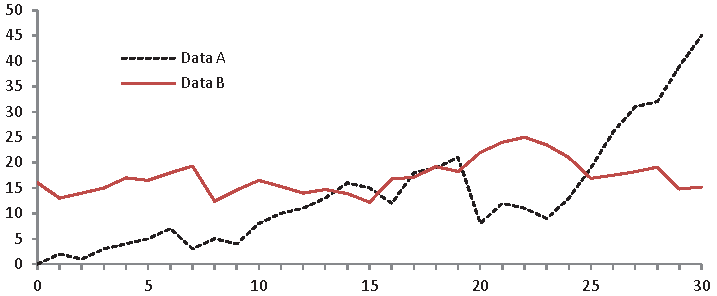
\includegraphics[width=\textwidth]{figures/fig1}
\caption{A figure caption is always placed below the illustration.
Please note that short captions are centered, while long ones are justified by the macro package automatically.} 
\label{fig1}
\end{figure}

\begin{theorem}
This is a sample theorem. 
The run-in heading is set in bold, while the following text appears in italics. 
Definitions, lemmas, propositions, and corollaries are styled the same way.
\end{theorem}
%
% the environments 'definition', 'lemma', 'proposition', 'corollary',
% 'remark', and 'example' are defined in the LLNCS documentclass as well.
%
\begin{proof}
Proofs, examples, and remarks have the initial word in italics, while the following text appears in normal font.
\end{proof}
For citations of references, we prefer the use of square brackets and consecutive numbers. 
Citations using labels or the author/year convention are also acceptable. 
The following bibliography provides a sample reference list with entries for journal articles~\cite{Stol2016}, a book~\cite{Myers2012}, conference proceedings~\cite{Harrold1988}, and a web site~\cite{Schaffer2018}.

\subsection{Abbreviations}
\label{sec:intro:sub:abbrev}

To use acronyms in the document, simple declare them in the main.tex file and use them later.
For example, you might want to define \acp{rq}, which will then be always abbreviated as \ac{rq} for singular or \acp{rq} for plural.

List are also really easy to create:

\begin{itemize}
  \item One entry in the list
  \item Another entry in the list
\end{itemize}

\begin{enumerate}
  \item The labels consists of sequential numbers.
  \item The numbers starts at 1 with every call to the enumerate environment.
\end{enumerate}

\subsection{Code Listings}
\label{sec:intro:sub:code}

Listings can either be created inside the text or imported:\footnote{See \url{https://www.overleaf.com/learn/latex/Code_listing} for a complete example.}
\begin{lstlisting}[language=C]
int main(int argc, char* argv[]) {
  return 0;
}
\end{lstlisting}
% !TeX spellcheck = en_US

\section{Related Work}
\label{sec:related_work}

In general, we can subdivide this section in two categories. First, existing works searching for the reasons for code clones in human, organizational and technological factors are examined and secondly, we focus on papers describing explicitly the correlation between certain languages and the appearance of code clones.

\subsection{Reasons for Code Clones}
\label{sec:reasons_for_code_clones}

\subsubsection{Human \& Organizational Factors}

Before describing how the choice of programming language can affect clones, we start with a brief overview on other reasons for clones. Here, first to mention are human factors like inadvertently or impatiently copying because time or understanding are missing. Missing abstraction and contrary the need to fulfill certain coupling and cohesion properties are also potential sources of generating code clones \cite{kasper2006cloning}.
The intention to minimize the risks when adopting new ideas in software are also driver for cloning code since this technique allows to keep errors through the introduced redundancy in just a single module \cite{cordy2003comprehending}. Further as time-to-market is critical, cloning can improve the speed of developing an early prototype, as analyzed by \cite{rajapakse2007using} for web-applications.

\subsubsection{Technological Factors}

Alongside these human and economic factors are standing "[t]echnology limitations" \cite{kasper2006cloning} like the utilization of a specific programming language.
\textit{Templating} is major feature of modern programming languages like \texttt{C++}, in contrast languages like \texttt{C} do not offer any equivalent feature. Given a certain algorithm working with double precision in the \texttt{C} programming language, the developer is forced to copy the procedure and replace "\texttt{double}" with "\texttt{float}". Such "boiler-plating [is enforced only] due to language inexpressiveness" \cite{kasper2006cloning}. 
Next to those more direct issues with Templating/ generalization in certain languages are keywords, standard library, and patterns how to fulfill certain tasks. For example, creating a \texttt{socket} and communicating with it varies and is different in each programming language - sometimes shorter, sometimes more lengthy, but usual there is one optimal way of doing it, so that possible exception (if the languages even has such a feature) or error codes are handled. These optimal sequences will then be often copy-and-pasted by developers \cite{kasper2006cloning}.
Further next to \textit{templating}, Kasper et. al. \cite{kasper2006cloning} mentions \textit{customization} as reasons for duplication. Code ownership can make bug fixing difficult, only allowing the creation of a work-around by copying and improving the faulty lines. Further, they number the idiom of "replicate and specialize", in which developers clone code to specialize a solution rather than generalizing an existing an implementation.
Lastly, Kasper et. al. \cite{kasper2006cloning} describe \textit{exact matches}, in context of code clones, as a result of copying "semantic properties [of] otherwise unrelated functionality" \cite{kasper2006cloning} between methods like logging or debugging statements and reusing certain code structures like loops which are easier copied than implemented as reusable function.

\subsection{Similar Analyses}
\label{sec:similiar_analyses}

This work will later present a comparison of clone coverage in different generation programming languages, but there are already some studies with a similar scope.

\subsubsection{Code Clones in Build Systems}

Once developer produced the different components of a large-scale software system, they typically need to be assembled together. This critical step usually accomplished with certain build systems like \texttt{Ant}, \texttt{Maven}, \texttt{Autotools} or \texttt{CMake} for respectively \texttt{Java} and \texttt{C/C++}. \cite{mcintosh2014collecting} compares these build systems with surprising results. As overall result, "build systems tend to have higher cloning rates than other software artifacts" \cite{mcintosh2014collecting}. 
They conclude with the finding that, as opposed of what one might think, modern build systems like \texttt{CMake} and \texttt{Maven} have higher clone coverage then their older counterparts and the \texttt{C/C++} systems and vice-versa \texttt{Java} build systems have a higher clone coverage, in many cases more than $50\%$, than the respective \texttt{C/C++} counterparts.

\subsubsection{Comparison of Java \& Scala}

Jorge et. al. \cite{jorge2012impact} directly compares features of the two languages \texttt{Java} and \texttt{Scala} and studies how their language constructs correlate to code cloning. In their findings, they conclude that code duplication problems arise with higher probability if a language is more verbose, e.g. due to getters and setters, anonymous classes, constructors, and lacks (simple) abstraction capabilities. Properties which finally lead to more effort refactoring code than simply cloning a source code. \cite{jorge2012impact}

% !TeX spellcheck = en_US

\section{Research Question}
\label{sec:research_question}

After introducing the topic, the following research questions may arise which are covered in this work:

\begin{enumerate}
	\item Which programming languages suffer mostly from high clone coverage?
	\item Do modern programming languages have lower clone coverage compared to older languages?
	\item Can we infer that a simpler, less verbose programming language always leads to less code clones?
\end{enumerate}

Important to note is that a question analyzing the "Why?" is missing since the following case study relies on quantitatively measuring code clone coverage in thousands of projects by just examining the source code, but not concrete software engineering process, i.e. principles of those projects. Rather \autoref{sec:results} will show certain trends for specific programming languages which are then discussed based on the formulated research questions in \autoref{sec:discussion}.
% !TeX spellcheck = en_US

\section{Study Design}
\label{sec:study_design}


\subsection{Overview}

\begin{figure}[htb]
	\label{fig:overview_deployment}
	\centering
	\includegraphics[width=\linewidth]{figures/setup/Code-Clone-Analysis-Deployment}
	\caption{UML Deployment Diagram of the presented examination}
\end{figure}

\begin{figure}[htb]
	\label{fig:overview_communication}
	\centering
	\includegraphics[width=\linewidth]{figures/setup/Code-Clone-Analysis-Communication}
	\caption{Diagram showing every processing step in order and associated data flow}
\end{figure}

\subsection{Implementation}
% !TeX spellcheck = en_US

\section{Results}
\label{sec:results}

This section now provides the results and a brief description of the previously presented study design. 


A first overview is given in \autoref{fig:overview_results}, which plots the clone coverage in dependence to the project size, i.e. the \acl{sloc}, for all analyzed projects. Further, the plot contains a trend line for each programming language in order to enable better comparability. These trend lines depict the mean value of clone coverage for every programming language until around $10^6$ of \ac{sloc} pretty close. Also, they clearly show that bigger projects tend to have a greater clone coverage.
Nevertheless, the data far beyond $10^6$ \acl{sloc} should be taken with caution since for some programming languages since not enough data could be collected for this size regime. 
\autoref{fig:overview_numbers} portrays this situation with the tick $10^6$ \ac{sloc} being marked since before $10^6$, we have at least 100 projects for every programming language, whereas languages like \texttt{Kotlin} and \texttt{Rust} only have small amounts of samples for e.g. more than $10^7$ \ac{sloc}.

\begin{figure}[tbh!]
	\centering
	\includegraphics[width=0.85\linewidth]{figures/results/scatter_clone_coverage_loc_m}
	\caption{Clone Coverage depending on projects' \ac{sloc} with trend lines plotted}
	\label{fig:overview_results}
\end{figure}

\begin{figure}[tbh!]
	\centering
	\includegraphics[width=0.85\linewidth]{figures/results/number}
	\caption{Complementary cumulative distribution function for the number of projects given a certain \ac{sloc} threshold}
	\label{fig:overview_numbers}
\end{figure}

In contrast, \autoref{fig:histo_all} shows the histograms of code clone coverage for every examined programming language.


Supplementary, \autoref{fig:histo_million} narrows this down to just presenting projects with more than one million \acl{sloc}. As previously mentioned, one million \ac{sloc} is the range where still enough data is present for some adequate evidence.

\begin{figure}[p]
	\centering
	\begin{subfigure}[t]{0.49\textwidth}
		\includegraphics[width=\textwidth]{figures/results/c/histogram_all}
		\caption{for pure \texttt{C}}
		\label{fig:histo_all_c}
	\end{subfigure}
	\hfill
	\begin{subfigure}[t]{0.49\textwidth}
		\includegraphics[width=\textwidth]{figures/results/cpp/histogram_all}
		\caption{for \texttt{C/C++}}
		\label{fig:histo_all_cpp}
	\end{subfigure}
	\begin{subfigure}[t]{0.49\textwidth}
		\includegraphics[width=\textwidth]{figures/results/rust/histogram_all}
		\caption{for \texttt{Rust}}
		\label{fig:histo_all_rust}
	\end{subfigure}
	\begin{subfigure}[t]{0.49\textwidth}
		\includegraphics[width=\textwidth]{figures/results/python/histogram_all}
		\caption{for \texttt{Python}}
		\label{fig:histo_all_python}
	\end{subfigure}
	\begin{subfigure}[t]{0.49\textwidth}
		\includegraphics[width=\textwidth]{figures/results/java/histogram_all}
		\caption{for \texttt{Java}}
		\label{fig:histo_all_java}
	\end{subfigure}
	\begin{subfigure}[t]{0.49\textwidth}
		\includegraphics[width=\textwidth]{figures/results/kotlin/histogram_all}
		\caption{for \texttt{Kotlin}}
		\label{fig:histo_all_kotlin}
	\end{subfigure}
	\begin{subfigure}[t]{0.49\textwidth}
		\includegraphics[width=\textwidth]{figures/results/go/histogram_all}
		\caption{for \texttt{Go}}
		\label{fig:histo_all_go}
	\end{subfigure}
	\caption{Histograms of the clone coverage distribution for the seven examined programming languages containing all project. Each plot contains the mean value and the standard deviation.}
	\label{fig:histo_all}
\end{figure}


\begin{figure}[p]
	\centering
	\begin{subfigure}[t]{0.49\textwidth}
		\includegraphics[width=\textwidth]{figures/results/c/histogram_million}
		\caption{for pure \texttt{C}}
		\label{fig:histo_million_c}
	\end{subfigure}
	\hfill
	\begin{subfigure}[t]{0.49\textwidth}
		\includegraphics[width=\textwidth]{figures/results/cpp/histogram_million}
		\caption{for \texttt{C/C++}}
		\label{fig:histo_million_cpp}
	\end{subfigure}
	\begin{subfigure}[t]{0.49\textwidth}
		\includegraphics[width=\textwidth]{figures/results/rust/histogram_million}
		\caption{for \texttt{Rust}}
		\label{fig:histo_million_rust}
	\end{subfigure}
	\begin{subfigure}[t]{0.49\textwidth}
		\includegraphics[width=\textwidth]{figures/results/python/histogram_million}
		\caption{for \texttt{Python}}
		\label{fig:histo_million_python}
	\end{subfigure}
	\begin{subfigure}[t]{0.49\textwidth}
		\includegraphics[width=\textwidth]{figures/results/java/histogram_million}
		\caption{for \texttt{Java}}
		\label{fig:histo_million_java}
	\end{subfigure}
	\begin{subfigure}[t]{0.49\textwidth}
		\includegraphics[width=\textwidth]{figures/results/kotlin/histogram_million}
		\caption{for \texttt{Kotlin}}
		\label{fig:histo_million_kotlin}
	\end{subfigure}
	\begin{subfigure}[t]{0.49\textwidth}
		\includegraphics[width=\textwidth]{figures/results/go/histogram_million}
		\caption{for \texttt{Go}}
		\label{fig:histo_million_go}
	\end{subfigure}
	\caption{Histograms of the clone coverage distribution for the seven examined programming languages containing only projects with at least one million \ac{sloc}. Each plot contains the mean value and the standard deviation.}
	\label{fig:histo_million}
\end{figure}
% !TeX spellcheck = en_US
\section{Discussion}
\label{sec:discussion}

\autoref{sec:results} has shown that the in \autoref{sec:study_design} presented approach for quantitatively measuring clone coverage in different programming languages is capable of answering some of the asked \aclp{rq}. This section will discuss and explain the observed results and evaluate the used approach.

\subsection{Implications of the result}

%Can we infer that a simpler, less verbose, more modern programming language always leads to less code clones?

At the outset, the extracted data does not imply that a particular programming language, e.g., \texttt{Python}, which performed best, should be used for every project. 
However, the results show that specific languages, \texttt{Python}, \texttt{Kotlin}, and \texttt{Rust}, performed significantly better than \texttt{C/C++} or \texttt{Java} and, therefore, seem to have advantages over the others.
One reason for fewer clones could be a less verbose, more straightforward programming language design, as discussed in \autoref{sec:similiar_analyses}, yet this argument can be partially discarded since \texttt{Go} performs for projects bigger than $10^6$ \ac{sloc}, similarly to \texttt{Java} and \texttt{C/C++}, although \texttt{Go} has the smallest set of keywords - implying simplicity, as depicted in \autoref{tab:keyword_number}.

\begin{table}[tbh!]
	\centering
	\begin{tabular}{|>{\centering\arraybackslash}m{2cm}|>{\centering\arraybackslash}m{1.5cm}|>{\centering\arraybackslash}m{1.5cm}|>{\centering\arraybackslash}m{1.5cm}|>{\centering\arraybackslash}m{1.5cm}|>{\centering\arraybackslash}m{2cm}|>{\centering\arraybackslash}m{1.5cm}|}
		\hline
		C/C++ 17 & Kotlin 1.4 & Rust 1.46 & Java 14 & C18 & Python 3.8 & Go 1.15 \\
		\hline
		84 & 79 & 53 & 51 & 44 & 35 & 25 \\
		\hline
	\end{tabular}
	\caption{Number of keywords for each examined programming language \cite{meyer2022keywords}}
	\label{tab:keyword_number}
\end{table}

Further, \autoref{sec:similiar_analyses} already introduced build systems as crucial for project success. Here might be another reason located. Simple to use package managers make importing existing solutions much more effortless, thereby preventing \textit{Reinventing the wheel}, a.k.a copying existing solutions. \texttt{Rust} and \texttt{Python} come with package managers \texttt{cargo} and \texttt{pip}, making the use of existing solutions much more manageable. In comparison, \texttt{C/C++} and \texttt{Java} rely on build systems like \texttt{CMake} and \texttt{Maven}, usually with a high learning curve. For example, to include a simple package/ library in \texttt{Python}, one must install and import it, whereas, in \texttt{CMake}, far more effort would be needed.

Lastly, one does not forget that, e.g., \texttt{Kotlin} and \texttt{Rust} improve \texttt{Java} and \texttt{C/C++}, respectively introducing null-safety and ownership. Thus these improvements avoid redundant, often repeated runtime checks like mentioned in \autoref{sec:reasons_for_code_clones} (reusing certain code structures).

Despite these reasons, the difference in mean clone coverage does not necessarily indicate that the programming language has flaws.
Older projects often have a greater (legacy) code base, which already can contain clones and makes it easy to copy and paste from there. 
However, \texttt{Rust}, \texttt{Kotlin}, and \texttt{Go} projects cannot be yet as old as projects in \texttt{C/C++} or \texttt{Java}. Consequently, the newer programming languages have some "time" advantage over the older ones, with projects having fewer developer changes and less legacy code.

In conclusion, we can finalize with the strong empirical suspect, but with no absolute certainty, that \texttt{Python}, \texttt{Kotlin}, and \texttt{Rust} are better designed to prevent code cloning than \texttt{C/C++}, \texttt{Java}, and \texttt{Go}, especially for larger projects with more extensive code bases.

 
\subsection{Threads to validity}

As the section above finalizes this work's conclusion, it is also required to include potential distortions.

First, the \textit{awesome lists} are different in size and contain different content for every programming language. Numerous contributors created them. Nonetheless, we have little information about why exactly something is on the list. So it is likely, that each list contains a certain bias. Additionally, the lists can also incorporate repositories containing only code snippets and similar utilities. The expressive analysis for more than $10^6$ \ac{sloc} should ensure that such projects are excluded, but a residual risk remains.

Directly related to this, the programming projects originate all from \textit{GitHub} and are publicly available. This circumstance is definitely a bias, since our study is not able to cover proprietary code nor big projects hosted on a different source.

The most considerable bias could be the evolution of programming languages. Writing modern \texttt{C++20} follows different guidelines than writing \texttt{C++98}. This behaves analogously to \texttt{Java} and \texttt{Python}. However, the study does not include when the projects were initially written and if they were refactored.

Lastly, $5224$ projects of only seven different programming languages were analyzed, which is, of course, only a tiny fraction at all.

\subsection{Future Work}

Directly related to the previous lessons of this section, future work could improve the solution by extending the scale of investigated projects and the concrete source. For example, a discarded approach for this work was the inclusion of projects from \textit{GitHub} with a certain amount of stars. The inclusion of projects from sources other than \textit{GitHub} or actually including examples from, e.g., a company with projects in different programming languages would also be of interest.

Further, independent validation of these results with another toolchain or another code clone detector than \teamscale{} is also thinkable.

A more qualitative approach could also be undertaken. Here, one could analyze only specific projects in more detail, like logging frameworks which usually exist in nearly every programming language and have similar functionality.
 

% !TeX spellcheck = en_US

\section{Conclusion}
\label{sec:conclusion}

\autoref{sec:intro} gave some first impressions about the difficulties in defining quality and quality properties and showed that it usually depends on the context. Next, \autoref{sec:related_work} portrayed the reasons for the emergence of code clones and presented investigations for code clones in build systems, as well as a comparison between \texttt{Java} and \texttt{Scala}.

Since there has been no quantitative approach to comparing code clone coverage across different programming languages, \autoref{sec:research_question} and \autoref{sec:study_design} presented a toolchain, using \teamscale{} as code clone detector, capable of answering these questions in \autoref{sec:results}:
\begin{enumerate}
	\item Which programming language has the lowest (mean) clone coverage?
	
	\mybox{\linewidth}{\texttt{Python} has a significant lower mean clone coverage than any of the other examined languages: pure \texttt{C}, \texttt{C/C++}, \texttt{Java}, \texttt{Kotlin}, \texttt{Rust}, \texttt{Go}.}
	
	\item Do modern programming languages have lower (mean) clone coverage than older ones?
	
	\mybox{\linewidth}{It depends, \texttt{Python} is a old programming language, but it performs in terms of clone coverage way better than the comparably new \texttt{Go}. On the other hand, \texttt{Kotlin} and \texttt{Rust} perform better than their older counterparts.}
	
	\begin{enumerate}
		\item Does pure \texttt{C} generally have a higher clone coverage than \texttt{C/C++}?
		
		\mybox{\linewidth}{No, since there is no significant difference in the mean values between \texttt{C} \texttt{C/C++}. Further, a KS test showed that both clone coverage distributions are equal.}
		
		\item Does \texttt{Rust} improve \texttt{C/C++} in terms of clone coverage?
		
		\mybox{\linewidth}{Yes, the study gave significant evidence that the mean clone coverage value of \texttt{C/C++} projects is greater than the mean of \texttt{Rust} projects.}
		
		\item Does \texttt{Kotlin} improve \texttt{Java} in terms of clone coverage?
		
		\mybox{\linewidth}{Yes, the study gave significant evidence that the mean clone coverage value of \texttt{Java} projects is greater than the mean of \texttt{Kotlin} projects.}
	\end{enumerate}
\end{enumerate}

In the end, we concluded with the verdict that there is strong empirical evidence that \texttt{Python}, \texttt{Kotlin}, and \texttt{Rust} are better designed to prevent code cloning than \texttt{C/C++}, \texttt{Java}, and \texttt{Go}. This finding can be the motivation for further validation by future studies and the foundation for additional examinations exploring code clones in different programming languages.
%
% ---- Appendix ----
%
\appendix
\section{Appendix}
\label{sec:appendix}

Anything additional goes here \dots
%
% ---- Bibliography ----
%
\bibliographystyle{splncs04}
\bibliography{library}
%
\end{document}
%
% ---- Begin Document ----
%
